\documentclass[letterpaper]{article}
\usepackage[margin=1in]{geometry}
\usepackage[utf8]{inputenc}
\usepackage{textcomp}
\usepackage{amssymb}
\usepackage{natbib}
\usepackage{graphicx}
\usepackage{gensymb}
\usepackage{amsthm, amsmath, mathtools}
\usepackage[dvipsnames]{xcolor}
\usepackage{enumerate}
\usepackage{mdframed}
\usepackage[most]{tcolorbox}
\usepackage{csquotes}
% https://tex.stackexchange.com/questions/13506/how-to-continue-the-framed-text-box-on-multiple-pages

\tcbuselibrary{theorems}

\newcommand{\R}{\mathbb{R}}
\newcommand{\Z}{\mathbb{Z}}
\newcommand{\N}{\mathbb{N}}
\newcommand{\Q}{\mathbb{Q}}
\newcommand{\C}{\mathbb{C}}
\newcommand{\code}[1]{\texttt{#1}}
\newcommand{\mdiamond}{$\diamondsuit$}
\newcommand{\PowerSet}{\mathcal{P}}
\newcommand{\Mod}[1]{\ (\mathrm{mod}\ #1)}
\DeclareMathOperator{\lcm}{lcm}

%\newtheorem*{theorem}{Theorem}
%\newtheorem*{definition}{Definition}
%\newtheorem*{corollary}{Corollary}
%\newtheorem*{lemma}{Lemma}
\newtheorem*{proposition}{Proposition}


\newtcbtheorem[number within=section]{theorem}{Theorem}
{colback=green!5,colframe=green!35!black,fonttitle=\bfseries}{th}

\newtcbtheorem[number within=section]{definition}{Definition}
{colback=blue!5,colframe=blue!35!black,fonttitle=\bfseries}{def}

\newtcbtheorem[number within=section]{corollary}{Corollary}
{colback=yellow!5,colframe=yellow!35!black,fonttitle=\bfseries}{cor}

\newtcbtheorem[number within=section]{lemma}{Lemma}
{colback=red!5,colframe=red!35!black,fonttitle=\bfseries}{lem}

\newtcbtheorem[number within=section]{example}{Example}
{colback=white!5,colframe=white!35!black,fonttitle=\bfseries}{def}

\newtcbtheorem[number within=section]{note}{Important Note}{
        enhanced,
        sharp corners,
        attach boxed title to top left={
            xshift=-1mm,
            yshift=-5mm,
            yshifttext=-1mm
        },
        top=1.5em,
        colback=white,
        colframe=black,
        fonttitle=\bfseries,
        boxed title style={
            sharp corners,
            size=small,
            colback=red!75!black,
            colframe=red!75!black,
        } 
    }{impnote}
\usepackage[utf8]{inputenc}
\usepackage[english]{babel}
\usepackage{fancyhdr}
\usepackage[hidelinks]{hyperref}

\pagestyle{fancy}
\fancyhf{}
\rhead{CSE 100}
\chead{September 28th, 2021}
\lhead{Course Notes}
\rfoot{\thepage}

\setlength{\parindent}{0pt}

\begin{document}

\begin{titlepage}
    \begin{center}
        \vspace*{1cm}
            
        \Huge
        \textbf{CSE 100 Notes}
            
        \vspace{0.5cm}
        \LARGE
        Advanced Data Structures
            
        \vspace{1.5cm}
            
        \vfill
            
        Fall 2021\\
        Taught by Professor Niema Moshiri
    \end{center}
\end{titlepage}

\pagenumbering{gobble}

\newpage 

\pagenumbering{gobble}
\begingroup
    \renewcommand\contentsname{Table of Contents}
    \tableofcontents
\endgroup

\newpage
\pagenumbering{arabic}


% ======================================================== %
%                   NEW SECTION                            %
% ======================================================== %
\section{A Brief Introduction}
In this course, we will primarily be building off of our prior knowledge of data structures (CSE 12). In particular, we will: 
\begin{itemize}
    \item Analyze data structures for both time and space complexity. 
    \item Describe the strengths and weaknesses of a data structure. 
    \item Implement complex data structures correctly and efficiently. 
\end{itemize}


% https://www.youtube.com/watch?v=_vpy1Flh__4&list=PLM_KIlU0WoXmkV4QB1Dg8PtJaHTdWHwRS&index=2
\subsection{Data Structures vs. Abstract Data Types}
When talking about data, we often hear about data structures and abstract data types. 

\begin{center}
    \begin{tabular}{|p{7cm}|p{7cm}|}
        \hline 
        \textbf{Data Structures} (DS) & \textbf{Abstract Data Type} (ADT) \\
        \hline 
        Data structures are collections that contain: 
        \begin{itemize}
            \item Data values. 
            \item Relationships among the data. 
            \item Operations applied to the data. 
        \end{itemize}
        It also describes how the data are organized and how tasks are performed. So, a data structure defines every single detail about anything relating to the data. 
        &
        Abstract data types are defined primarily by its \underline{behavior} from the view of the \underline{user}. So, not necessarily how the operations are done, but rather what operations it must have from a completely abstract point of view.  
    
        \bigskip 
    
        Specifically, it describes only what needs to be done, not how it's done. \\
        \hline 
    \end{tabular}
\end{center}

Consider the \code{ArrayList} (DS) vs. the \code{List} (ADT).
\begin{itemize}
    \item A \code{List} will most likely have the following operations: 
    \begin{itemize}
        \item \code{add}: Adds an element to the list.
        \item \code{find}: Does an element exist in the list? 
        \item \code{remove}: Remove an element from the list. 
        \item \code{size}: How many elements are in this list? 
        \item \code{ordered}: Each element should be ordered in the way we added it. For example, if we added \code{5}, and \emph{then} added \code{3}, and \emph{then} added \code{10}, our list should look like: \code{[5, 3, 10]}.   
    \end{itemize}

    Of course, as an abstract data type, \code{List} isn't going to define how these operations work. It just lists all operations that any implementing data structure must have. In other words, we can think of \code{List}, or any abstract data type, as a \emph{blueprint} for future data structures. 

    \item An \code{ArrayList} is simply an array that is expandable. It is internally backed by an \underline{array}. So, we can perform the following operations: 
    \begin{itemize}
        \item We can \code{add} an element to the \code{ArrayList}. In this case, we add the element to the next available slot in the array, expanding the array if necessary. 
        \item We can \code{find} an element in the \code{ArrayList}. In this case, we can search through each slot of the array until we find the array or we reach the end of the array.
        \item We can \code{remove} an element from the \code{ArrayList}. In this case, we can simply move every element after the specified element back one slot. 
        \item We can get the \code{size} of the \code{ArrayList}. In this case, this is as simple as seeing how many elements are in this \code{ArrayList}.
        \item And, we know that the \code{ArrayList} is \code{ordered}. In this case, this is already done via the \code{add} and \code{remove} methods.  
    \end{itemize}
    Notice how \code{ArrayList} specifies how each operation defined by \code{List} works. In this sense, we say that \code{ArrayList} essentially implements \code{List} because we need to define \emph{how} the tasks defined by \code{List} are performed. 
\end{itemize}
So, the key takeaways are: 
\begin{itemize}
    \item An abstract data type (in our case, \code{List}) specifies what needs to be done without specifying how it's done. 
    \item A data structure (in our case, \code{ArrayList}) actually defines \textbf{how} the data is organized, how the different operations are performed, and how exactly everything is represented.
\end{itemize}











% ======================================================== %
%                   NEW SECTION                            %
% ======================================================== %
\newpage 
\section{Introduction to C++}
Here, we will talk about C++, the programming language that we will use in this course. 

% https://www.youtube.com/watch?v=8FGvlugzS5A&list=PLM_KIlU0WoXmkV4QB1Dg8PtJaHTdWHwRS&index=4
\subsection{Data Types}
First, we'll compare the data types in Java and C++. 
\begin{center}
    \begin{tabular}{|c|c|c|}
        \hline 
        \textbf{Data Type} & \textbf{Java} & \textbf{C++} \\ 
        \hline 
        \code{byte} & 1 byte & 1 byte \\ 
        \code{short} & 2 bytes & 2 bytes \\ 
        \code{int} & 4 bytes & 4 bytes \\ 
        \code{long} & 8 bytes & 8 bytes \\ 
        \code{long long} & & 16 bytes \\ 
        \hline 
        \code{float} & 4 bytes & \code{4 bytes} \\ 
        \code{double} & 8 bytes & \code{8 bytes} \\ 
        \hline 
        \code{boolean} & Usually 1 byte & \\ 
        \code{bool} &  & Usually 1 byte \\ 
        \code{char} & 2 bytes & 1 byte \\ 
        \hline 
    \end{tabular}
\end{center}
It should be mentioned that: 
\begin{itemize}
    \item In Java, you can only have signed data types. 
    \item In C++, you can have both signed and unsigned data types. 
    \item \code{boolean} (Java) and \code{bool} (C++) are effectively the same thing: they represent either \code{true} or \code{false}. 
\end{itemize}

\subsection{Strings}
There are some major differences between strings in Java and C++, which we will discuss below.

\subsubsection{Representation}
In Java, strings are represented by the \code{String} class. In C++, strings are represented by the \code{string} type.

\subsubsection{Mutability}
Strings in Java are \underline{immutable}. The moment you create a string, you won't be able to modify them. The only way to change a string variable is by creating a new string and reassigning them. 

\bigskip 

In C++, strings are actually \underline{mutable}. You can modify strings in-place. 

\subsubsection{Concatenation}
In Java, you can concatenate any type to a string. For example, the following is valid:
\begin{verbatim}
    String a = "this is a string" + 123;\end{verbatim}

In C++, you can only concatenate strings with other strings. So, if you wanted to convert an integer (or any other type) to a string, you would have to \emph{first} convert that integer to a string (or use a string stream).

\subsubsection{Substring Method}
In Java, we can take the substring of a string using the \code{substring} method. The method signature is:
\begin{verbatim}
    String#substring(beginIndex, endIndex);\end{verbatim}

In C++, we can take the substring using the \code{substr} method. The method signature is:
\begin{verbatim}
    string#substr(beginIndex, length);\end{verbatim}

An important distinction to make here is that Java's \code{substring} method takes in an \textbf{end index} for the second parameter, whereas C++'s \code{substr} method takes in a \textbf{length} for the second parameter.



\subsection{Comparing Non-Primitive Objects}
Suppose \code{a} and \code{b} are two non-primitive objects.

\bigskip 

In Java, if we want to compare these two objects, we have to make use of the methods: 
\begin{verbatim}
    a.equals(b)
    a.compareTo(b)
\end{verbatim}
If we tried using the relational operators like \code{==} or \code{!=}, Java would compare the memory addresses of the two objects, which is often something that we aren't looking for.

\bigskip 

In C++, even if \code{a} and \code{b} are objects, we can make use of the relational operators:
\begin{verbatim}
    a == b      a != b
    a < b       a <= b
    a > b       a >= b
\end{verbatim}
This is done through something called \textbf{operator overloading}, where we write a custom class and define how these operators should function.


\subsection{Variables}
Now, we will briefly discuss how variables function in both C++ and Java. 

\subsubsection{Initialization}
In Java, variable initialization is \textbf{checked}. Consider the following code: 
\begin{verbatim}
    int fast;
    int furious; 
    int fastFurious = fast + furious;
\end{verbatim}
Because \code{fast} and \code{furious} aren't initialized, the Java compiler will throw a compilation error. 

\bigskip 

In C++, variable initialization is \textbf{not checked}. Consider the same code, which will compile:
\begin{verbatim}
    int fast;
    int furious; 
    int fastFurious = fast + furious;
\end{verbatim}
Here, this would result in \textbf{undefined} behavior.

\subsubsection{Narrowing}
In Java, if we have a higher variable type and then try to cast this type to a smaller type, we would get a compilation error. Consider the following code:
\begin{verbatim}
    int x = 40_000;
    short y = x;
\end{verbatim}
This code would result in a compilation error. If we didn't want a compilation error, we would have to explicitly \emph{cast} the bigger variable type to the smaller type. The following Java code would compile just fine: 
\begin{verbatim}
    int x = 40_000;
    short y = (short) x;
\end{verbatim}

\bigskip 

In C++, no compilation error would occur; that is, the following code would compile:
\begin{verbatim}
    int x = 40_000;
    short y = x;
\end{verbatim}
What would actually happen is that \code{x} would get \textbf{truncated} when it is assigned to \code{y}, resulting in integer overflow. 


\subsubsection{Variable Declaration}
In Java, variables \textbf{cannot} be declared outside of a class. The following Java code would result in a compile error:
\begin{verbatim}
    // MyClass.java 

    int meaningOfLife = 42;
    class MyClass {
        // some code 
    }
\end{verbatim}
In order for this to compile, you have to put variable declarations inside the class space (as an instance variable) or in a method inside a class (as a local variable). 

\bigskip 

In C++, variables \textbf{can} be declared outside of a class. The following C++ code would compile completely fine: 
\begin{verbatim}
    // MyClass.cpp

    int meaningOfLife = 42;
    class MyClass {
        // some code 
    }
\end{verbatim}
Here, \code{meaningOfLife} is a \textbf{global variable}. Anything in this file can access this variable. In general, it is considered poor practice to use global variables except in cases of constants. 

\subsection{Classes, Source Code, and Headers}
Another thing that is important is the concept of classes (which leads to the topic of object-oriented programming). That being said, Java and C++ has some differences with regards to how classes function. 

\subsubsection{Class Declaration}
There are some key differences in how methods and instance variables are laid out in Java and C++. 

In Java, a typical class would look like: 
\begin{verbatim}
    class Student {
        public static int numStudents = 0;
        private String name; 
        
        public Student(String n) { /* Code */ }

        public void setName(String n) { /* Code */ }
        public String getName() { /* Code */ }
    }
\end{verbatim}

And in C++, a typical class would look like: 
\begin{verbatim}
    class Student {
        public: 
            static int numStudents; 

            Student(string n);
            
            void setName(string n);
            string getName() const; 

        private: 
            string name; 
    }

    int Student::numStudents = 0;
    Student::Student(string n) { /* Code */ }
    void Student::setName(string n) { /* Code */ }
    string Student::getName() const { /* Code */ }
\end{verbatim}

There are several notable differences: 
\begin{itemize}
    \item \textbf{Modifiers:} In Java, if you want your method or instance variable to have an access modifier, you explicitly state the access modifier. In C++, you have a region for your access modifier. That is, there is a \code{public} region, \code{private} region, etc. Any methods or instance variables listed under these regions will take on that access modifier. For instance, \code{setName} is in the \code{public} region, so \code{setName} is public.
    \item \textbf{Implementation:} In Java, directly after declaring a method or constructor in a class, we need to provide the implementation code. In C++, we can ``declare'' the methods and the constructor, and then outside of the class we can implement the methods.
\end{itemize}
Now, consider the following C++ code: 
\begin{verbatim}
    class Point {
        private: 
            int x; 
            int y;
        
        public:
            Point(int i, int j);
    }

    Point::Point(int i, int j) {
        x = i;
        y = j;
    }
\end{verbatim}
Here, we're initializing the \code{x} and \code{y} instance variables directly from the constructor implementation. However, we can initialize these instance variables directly like so: 
\begin{verbatim}
    class Point {
        private: 
            int x; 
            int y;
        
        public:
            Point(int i, int j);
    }

    Point::Point(int i, int j) : x(i), y(j) {}
\end{verbatim}
This is called the \textbf{member initializer list}.

\subsubsection{Source vs. Header Files}
Consider the following class: 
\begin{verbatim}
    class Student {
        public: 
            static int numStudents;
            Student(string n);
        
        private: 
            string name; 
    }

    int Student::numStudents = 0;
    Student::Student(string n) : name(n) {
        numStudents++;
    }
\end{verbatim}
We can choose to break this up into two separate files; a \textbf{source} (usually \code{.cpp}) file and a \textbf{header} (usually \code{.h}) file. The header file contains the class and the method \emph{declaration}; the source file contains the implementations for those methods. So, the above code can be written like so: 
\begin{verbatim}
    // The header file 
    // Student.h
    class Student {
        public: 
            static int numStudents;
            Student(string n);
        
        private: 
            string name; 
    }

    // The source file 
    // Student.cpp 
    int Student::numStudents = 0;
    Student::Student(string n) : name(n) {
        numStudents++;
    }
\end{verbatim}

\subsection{Memory Diagrams}
Consider the following Java code: 
\begin{verbatim}
    Student s1 = new Student("Niema");
    Student s2 = s1;
\end{verbatim}
Here, \code{s1} is a \emph{reference} to a \code{Student} object. This \code{Student} object contains a \emph{reference} to a \code{string} object with the content \code{Niema}. That is: 
\begin{verbatim}
    Student object
    |----------|
    | |----|   |   (Reference)  |-------|
    | |name|------------------> | Niema |
    | |----|   |                |-------|
    |----------|   <------      String object
       /|\                \
        |                  \
        |                   \ (Reference)
        |                   |
        | (Reference)       |
    s1 -/                   s2
\end{verbatim} 
It also follows that \code{s2} is a reference to the same object that \code{s1} is referring to. 

\bigskip 

Now, consider the following C++ code: 
\begin{verbatim}
    Student s1("Niema");
    Student s2 = s1;
\end{verbatim}
Here, \code{s1} is a \code{Student} \emph{object}. The \code{Student} object contains a \code{string} object with the content \code{Niema}. That is:
\begin{verbatim}
    |-----------------|     |-----------------|
    | |-----------|   |     | |-----------|   |
    | |name: Niema|   |     | |name: Niema|   |
    | |-----------|   |     | |-----------|   |
    |  string object  |     |  string object  |
    |-----------------|     |-----------------|
    Student object          Student object
       s1                       s2
\end{verbatim} 
Additionally, when we assign \code{s1} to \code{s2}, we actually make a copy of said object. So, \code{s2} is its own object; it does not share a reference with \code{s1}.

\bigskip 

In other words, in Java, \code{s1} and \code{s2} are both references to the same object; in C++, \code{s1} \emph{is} the object and \code{s2} is \emph{another} object.

\subsubsection{References}
Consider the following C++ code: 
\begin{verbatim}
    Student s1 = Student("Niema");
    Student & s2 = s1;
    Student s3 = s2;
\end{verbatim}
The memory diagram looks like this: 
\begin{verbatim}
    |-----------------|     |-----------------|
    | |-----------|   |     | |-----------|   |
    | |name: Niema|   |     | |name: Niema|   |
    | |-----------|   |     | |-----------|   |
    |  string object  |     |  string object  |
    |-----------------|     |-----------------|
    Student object          Student object 
       s1      s2               s3
\end{verbatim} 
Here, \code{s2} can be seen as \emph{another} way to call \code{s1} (think of \code{s2} as another name for \code{s1}). \code{s3} would be a copy of \code{s1}. 

\subsubsection{Pointers}
Pointers are similar to Java references. Consider the following C++ code: 
\begin{verbatim}
    Student s = Student("Niema");
    // * in this case means pointer 
    // & means memory address
    // So, ptr stores a memory address to some object. In other words, 
    // it points to the object s. 
    Student* ptr = &s; 
    Student** ptrPtr = &ptr; 
\end{verbatim}
The memory diagram would look like: 
\begin{verbatim}
    Mem. Address: 9500 
    |-----------------|
    | |-----------|   |       |-----------|       |-----------|
    | |name: Niema|   |  <--- |    9500   |  <--- |           |
    | |-----------|   |       |-----------|       |-----------|
    |  string object  |       Student* (pointer)   Student** (pointer to pointer) 
    |-----------------|           ptr                  ptrPtr
    Student object      
       s
\end{verbatim} 
If we wanted to access an object through a pointer, we can do this in several ways. 
\begin{enumerate}
    \item Deferencing a pointer. 
    \begin{verbatim}
        // * in this case dereferences the pointer
        // Think of the * as following the arrow  
        (*ptr).name; 
    \end{verbatim}

    \item Arrow dereferencing. 
    \begin{verbatim}
        // ptr->x is the same thing as (*ptr).x
        ptr->name; 
    \end{verbatim}
\end{enumerate}

\subsubsection{Memory Management}
Consider the following C++ code: 
\begin{verbatim}
    Student s1 = Student("Niema");
    Student* s2 = new Student("Ryan");
\end{verbatim}
The corresponding memory diagram is: 
\begin{verbatim}
    |-----------------|     |-----------------|
    | |-----------|   |     | |-----------|   |
    | |name: Niema|   |     | |name: Ryan |   |
    | |-----------|   |     | |-----------|   |
    |  string object  |     |  string object  |
    |-----------------|     |-----------------|
    Student object          Student object 
       s1                                 /|\
                                           |
                                           |
                                           |
                                |------|   |
                                |      | --/
                                |------|
                                Student* (pointer)
                                s2
\end{verbatim}
Here, \code{s1} is allocated on the \emph{stack}; once the method returns, \code{s1} is automatically destroyed. 

\bigskip 

\code{s2} is allocated through the \code{new} keyword. This is known as dynamic memory allocation. So, \code{s2} is a pointer to the newly allocated memory. Because this object was created using the \code{new} keyword, we need to deallocate it ourselves. To do so, we need to explicitly call \code{delete} on this object: 
\begin{verbatim}
    delete s2; 
\end{verbatim}
\code{delete} takes in a memory address (i.e. pointer). This is very similar to \code{free} (in C). If we don't free this, we run into what is called a \textbf{memory leak}. 

\subsection{Constant Keyword}
In C++, the \code{const} keyword means that the variable can never be reassigned. Consider the following: 
\begin{verbatim}
    const int a = 42; 
    int const b = 42;
\end{verbatim}
If we tried reassigning \code{a} (e.g. \code{a = 41;}), we would get a compiler error. 

\bigskip

The second line (\code{int const}) is identical to the first line. 


\subsubsection{\code{const} and Pointers}
Consider the following C++ code: 
\begin{verbatim}
    int a = 42;                     // a 
    const int* ptr1 = &a;           // b
    int const* ptr2 = &a;           // c
    int* const ptr3 = &a;           // d
    const int* const ptr4 = &a;     // e
\end{verbatim}
\begin{itemize}
    \item For lines (b) and (c), the pointer cannot modify the object that it is pointing to.  But, we can reassign the pointer to point to a different object. 
    \item For line (d), we cannot reassign the pointer to point to a different object. However, we can modify the object that the pointer is pointing to. 
    \item For (e), we cannot reassign the pointer to point to a different object \emph{or} modify the object that the pointer is pointing to. 
\end{itemize}
In general:
\begin{verbatim}
    const type* const varName = ...; 
    ----------- -------------
       (a)            (b)
\end{verbatim}
\begin{itemize}
    \item Segment (A): The \code{const} next to \code{type*} means that we cannot modify the object or value behind the pointer. 
    \item Segment (B): The \code{const} next to \code{varName} (the variable name) means that we cannot reassign the pointer to point to a different object or value. 
\end{itemize}

\subsubsection{\code{const} and References}
Suppose we have the following C++ code: 
\begin{verbatim}
    int a = 42; 
    const int & ref1 = a;       // a
    int const & ref2 = a;       // b
\end{verbatim}
\begin{itemize}
    \item In (a), the \code{const} means that we cannot modify the variable through the constant reference. So: 
    \begin{verbatim}
        a = 21;         // Allowed. 
        ref1 = 20;      // Compile error!
    \end{verbatim}

    \item (b) is the same exact thing is (a).
\end{itemize}

\subsubsection{\code{const} Functions}
Recall the \code{Student} class from earlier: 
\begin{verbatim}
    class Student {
        public: 
            Student(string n);
            string getName() const; 
            
        private: 
            string name; 
    }

    Student::Student(string n) : name(n) {}
    string Student::getName() const {
        return name;
    }
\end{verbatim}
What does the \code{const} in \code{getName()} do? Well, the \code{const} keyword after the function declaration means that the function cannot modify \emph{this} object. So: 
\begin{itemize}
    \item You cannot do any assignments to instance variables. 
    \item You can only call other \code{const} functions.
\end{itemize} 
So, effectively, \code{const} after a function name means that we are guaranteeing that we aren't changing the object's state in any way.

\subsection{Functions}
In C++, we can have global functions (functions that are defined outside of classes). For instance, the main method (shown below) is a global function (and is required to be):
\begin{verbatim}
    int main() {
        /* Do stuff */ 
    }

    class MyClass {
        /* Some code */ 
    }
\end{verbatim}

\subsubsection{Passing by Value vs. Reference}
In C++, you can pass parameters either by value or reference. 

\bigskip

When passing by value, the function makes a \textbf{copy} of the values that you passed in. Some example code is shown below:
\begin{verbatim}
    void swap(int a, int b) {
        int tmp = a;
        a = b;
        b = tmp;
    }
\end{verbatim}
These copies are destroyed once the function returns (the stack frame is destroyed). 

\bigskip 

When passing by reference, the function takes in \emph{references} to the variables. Some example code is shown below:
\begin{verbatim}
    void swap(int & a, int & b) {
        int tmp = a;
        a = b;
        b = tmp;
    }
\end{verbatim}
Effectively, whatever you change with the references will be reflected with the actual variables. So, in the above \code{swap} method, \code{a} and \code{b} will be updated after the function is done. 

\subsection{Vectors}
A C++ \code{vector} is very similar in nature to Java's \code{ArrayList} class and arrays. Consider the following code, which demonstrates some common operations: 
\begin{verbatim}
    // Creates a new vector. 
    vector<int> a; 
    // Adds 42 to end of vector. Looks like: [42]
    a.push_back(42);
    // Adds 21 to end of vector. Looks like: [42, 21]
    a.push_back(21);
    // Removes 21 from vector. Looks like [42] 
    a.pop_back(); // returns 21 
    // We can access the first element (0th index).
    a[0];
\end{verbatim}
Like Java arrays or \code{ArrayList}, elements in a C++ vector are stored contiguously; that is, they are stored after the previous element. 

\bigskip 

We know that if we assign an object to another variable, the other variable will get a full copy of that object. The same applies to vectors; we can also create a copy of a vector simply be reassigning it:
\begin{verbatim}
    vector<int> a;
    a.push_back(42);
    vector<int> b = a;
    // a: [42]
    // b: [42]
\end{verbatim}

\subsection{Input and Output}
Consider the following code: 
\begin{verbatim}
    int n; 
    cout << "Enter a number: "; 
    cin >> n; 

    string message; 
    cout << "Enter a message: "; 
    getline(cin, message);

    if (cin.fail()) {
        cerr << "Bad input!" << endl; 
    }
\end{verbatim}
Here: 
\begin{itemize}
    \item \code{cin} represents standard input (\code{stdin}). 
    \item \code{cout} represents standard output (\code{stdout}). 
    \item \code{cerr} represents standard error (\code{stderr}).
\end{itemize}
In C++, we can use \code{istream} to handle input stream and \code{ostream} to handle output stream. \code{cin} is an example of an \code{istream}; \code{cout} is an example of an \code{ostream}. 

\bigskip 

We can make use of the overloaded \code{<<} and \code{>>} operators to write to standard output and read from standard input, respectively. So: 
\begin{itemize}
    \item \code{cout << "Enter a number"} effectively means to write this message to standard output. 
    \item \code{cin >> n} effectively means to read from the standard input and store that input into \code{n}. We aren't necessarily restricted to \code{int}; we could use \code{long}, \code{double}, \code{string}, etc. 
    \item We can also use \code{getline} to read from standard input and then store the result into a variable. In our example above, we called \code{getline(cin, message)}. \code{cin} is where we are reading the input from and \code{message} is the variable where we store the result of reading from \code{cin}. 
    \item \code{endl} means \code{end} \code{l}ine and, in our use case here, writes a new line to standard error. In reality, we can use \code{endl} to write a newline to standard output or error.  
\end{itemize}

\subsection{Templates}
Templates introduce the notion of \emph{generic programming}. Consider the following code in Java: 
\begin{verbatim}
    class Node<Data> {
        public final Data data; 
        public Node(Data d) {
            data = d;
        }
    }

    Node<String> a = new Node<String>(s);
    Node<Integer> a = new Node<Integer>(s);
\end{verbatim}
The generic type is \code{Data} (though you can rename it to whatever you want). We can use this type either as a parameter type or a return type. When creating a new object with a generic type, we simply put the type between the \code{<>} (like with the \code{Node} examples).

\bigskip 

Consider the equivalent C++ example: 
\begin{verbatim}
    template<typename Data>
    class Node {
        public: 
            Data const data; 
            Node(const Data & d) : data(d) {}
    }

    Node<string> a(s);
    Node<int> b(n);
\end{verbatim}
Here, we can use templates to achieve similar results (compared to the Java example). Functionality-wise, this is similar to Java. 

\subsection{Iterators}
Consider the following C++ code: 
\begin{verbatim}
    for (string name : names) {
        cout << name << endl; 
    }
\end{verbatim}
What is \code{names}? 
\begin{itemize}
    \item Is it a \code{vector}? 
    \item Is it a \code{set}? 
    \item Is it an \code{unordered\_set}?
    \item Is it another collection that C++ has? 
\end{itemize}
Well, it doesn't matter! Regardless of what collection we are using, how we use it doesn't matter when it comes to iterating over it. This functionality is made possible by something called \textbf{iterators}.

\subsubsection{Iterating Over Arrays}
Consider the following code: 
\begin{verbatim}
    void printInorder(int* p, int size) {
        for (int i = 0; i < size; ++i) {
            cout << *p << endl; 
            ++p; 
        }
    }
\end{verbatim}
The \code{*p} deferences the pointer, giving the value at the location that the pointer is pointing to. 

\bigskip

The \code{++p} is an example of pointer arithmetic; this will add whatever the size of the type is to the pointer. In this case, this will make the pointer point to the memory address of the next element in the array. 

\bigskip 

Here, we know that \code{p} is (initially) a pointer to the first element in the array: 
\begin{verbatim}
     0   4   8   12  16  20  24  28         Memory Address 
     ------------------------------         (sizeof(int) = 4)
    [10, 20, 25, 30, 46, 50, 55, 60]        Array 
     ^
     p                                      Pointer 
\end{verbatim}
Dereferencing \code{p} (\code{*p}) gives us \code{10}. 

\bigskip 

When we do \code{++p}, we made the pointer point to the next memory address: 
\begin{verbatim}
    0   4   8   12  16  20  24  28         Memory Address 
    ------------------------------
   [10, 20, 25, 30, 46, 50, 55, 60]        Array 
        ^
        p                                  Pointer 
\end{verbatim}
Dereferencing \code{p} (\code{*p}) gives us \code{20}. 


\subsubsection{Using Iterators}
Consider the following C++ code: 
\begin{verbatim}
    vector<string> names; 
    // populate with data 

    vector<string>::iterator itr = names.begin(); 
    vector<string>::iterator end = names.end(); 
    
    while (itr != end) {
        cout << *itr << endl; 
        ++itr; 
    }
\end{verbatim}
Here, we note a few things. 
\begin{itemize}
    \item \code{iterator} is simply a class that handles, well, iteration. So, \code{itr} and \code{end} are instances of the \code{iterator} class that is iterating over \code{names}. 
    \item The \code{!=} operator (in \code{itr != end}) has been overloaded. This checks the \code{curr} property in the \code{iterator} class to see if it is equal (or, more specifically, not equal) to the \code{curr} property of the other index. In this case, \code{itr != end} is effectively comparing \code{itr.curr} with \code{itr.end}. 
    \item The \code{*} dereferencing operator (in \code{*itr}) has also been overloaded. This operator has been overloaded to return whatever the value is at the \code{curr} index. So, in our case,\code{*itr} would return whatever value is at the specified \code{curr} index in the array that we are iterating through. 
    \item The \code{++} operator (in \code{++itr}) is also overloaded. This will increment the \code{curr} property in the \code{iterator} instance. 
\end{itemize}

Suppose \code{names} has the following: 
\begin{verbatim}
        0       1       2           // Index 
    ["Niema", "Ryan", "Felix"]      // names array 
\end{verbatim}

Essentially, \code{vector<string>::iterator} will look something like: 
\begin{verbatim}
    |-----------------------------| |-----------------------------|
    |         |----|              | |         |----|              |
    |   curr: | 0  |              | |   curr: | 3  |              |
    |         |----|              | |         |----|              |
    |           int               | |           int               |
    |-----------------------------| |-----------------------------|
                itr                             end
\end{verbatim}
Calling \code{*itr} will basically give us \code{names[curr]} (or, more specifically, \code{names[0]}). Comparing \code{itr != end} is basically the same as checking \code{0 != 3}. 

\bigskip 

When we call \code{++itr}, we now have: 
\begin{verbatim}
    |-----------------------------| |-----------------------------|
    |         |----|              | |         |----|              |
    |   curr: | 1  |              | |   curr: | 3  |              |
    |         |----|              | |         |----|              |
    |           int               | |           int               |
    |-----------------------------| |-----------------------------|
                itr                             end
\end{verbatim}
Calling \code{*itr} now will basically give us \code{names[curr]} (or, more specifically, \code{names[1]}). Comparing \code{itr != end} is basically the same as checking \code{1 != 3}. 

\subsubsection{Linked List Iterator}
Consider the following code, which is essentially the same code as the previous one: 
\begin{verbatim}
    LinkedList<string> names; 
    // populate with data 

    LinkedList<string>::iterator itr = names.begin(); 
    LinkedList<string>::iterator end = names.end(); 
    
    while (itr != end) {
        cout << *itr << endl; 
        ++itr; 
    }
\end{verbatim}
The only difference is that we're now using a \code{LinkedList} instead of \code{vector}. However, the way the data is structured is very different. Suppose \code{names} has the following: 
\begin{verbatim}
    |---------------|      |---------------|      |---------------|
    | data: "Niema" |      | data: "Ryan"  |      | data: "Felix" |
    |     next: [ ] ---->  |     next: [ ] ---->  |     next: [x] |
    |---------------|      |---------------|      |---------------|
\end{verbatim}

Here, \code{[x]} (in the \code{next} property of the last node) is a \code{nullptr}. 

\bigskip

How does using nodes change our iterator? Well, \code{LinkedList<string>::iterator} will look something like: 
\begin{verbatim}
    |---------------|      |---------------|      |---------------|
    | data: "Niema" |      | data: "Ryan"  |      | data: "Felix" |
    |     next: [ ] ---->  |     next: [ ] ---->  |     next: [x] |
    |---------------|      |---------------|      |---------  /|\ |
               /|\                                             |
                |                                              |
                |                                  ------------/
                |                                 /  
                |                                /
    |-----------|-----------------| |------------|----------------|
    |         |-|--|              | |         |--|-|              |
    |   curr: |    |              | |   curr: |    |              |
    |         |----|              | |         |----|              |
    |         Node*               | |         Node*               |
    |-----------------------------| |-----------------------------|
                itr                             end
\end{verbatim}
Going back to the code: 
\begin{verbatim}
    while (itr != end) {
        cout << *itr << endl; 
        ++itr; 
    }
\end{verbatim}
It should be noted that: 
\begin{itemize}
    \item \code{!=} is once again overloaded to compare the values of the node's \code{data}. 
    \item \code{*itr} is once again overloaded to return \code{data}. It would look like: 
    \begin{verbatim}
        return curr->data;
    \end{verbatim}
    \item \code{++itr} is once again overloaded to make the iterator move to the next node. This would look like: 
    \begin{verbatim}
        curr = curr->next; 
    \end{verbatim}
\end{itemize}

\subsubsection{Creating an Iterator Class}
When creating data structures, we'll often need to create our own Iterator classes. 

\bigskip 

First, we'll talk about the operators associated with the iterator class: 
\begin{itemize}
    \item \code{==}: \code{true} if the iterators are pointing to the same item and \code{false} otherwise. 
    \item \code{!=}: \code{true} if the iterators are pointing to the different item and \code{false} otherwise. 
    \item \code{*} (dereference): Return a reference to the current data value. 
    \item \code{++} (pre- and post-increment): Move the iterator to the next item. 
\end{itemize}

And, we also need to talk about what functions are in the \underline{data structure class} so we can make use of the iterator:
\begin{itemize}
    \item \code{begin()}: Returns an iterator to the first element. 
    \item \code{end()}: Returns an iterator to the element just after the last element (not the last element, but \emph{after} the last element).  
\end{itemize}
So, in the Linked List example: 
\begin{verbatim}
    [] -> [] -> []
    ^              ^
    begin()        end()
\end{verbatim}
And in any array-based structures: 
\begin{verbatim}
    [a, b, c, d, e]
     ^              ^
     begin()        end()
\end{verbatim}


\newpage
\section{Time and Space Complexity}
One of the key things computer scientists try to do is automate competitive tasks, and of course, that requires \emph{performance}. So, that begs the question: how can we measure the performance of our program? 
\begin{itemize}
    \item How many hours does it take to run? 
    \item Minutes? 
    \item Nanoseconds? 
\end{itemize}
These are all metrics of \emph{human time}. However, a program has two aspects: 
\begin{itemize}
    \item The implementation. 
    \item The algorithm behind that program. 
\end{itemize}
While these different metrics of human time are good at measuring the actual implementation of a program, they don't do a good job describing how fast the \emph{idea}, the algorithm itself, is. For instance, running the algorithm on two different devices, both which have wildly different hardware, will result in a significant difference in how fast your algorithm runs. 

\bigskip 

That being said, we want to know how fast an algorithm is. The best way to do so is by figuring out the performance in terms of number of operations with respect to the input size $n$ (instead of the amount of time). 

\subsection{Notation of Complexity}
Consider the following notations: 
\begin{itemize}
    \item Big-$O$: Upper bound. 
    \item Big-$\Omega$: Lower bound. 
    \item Big-$\theta$: Both upper and lower bound. 
\end{itemize}
Consider the following graph: 
\begin{center}
    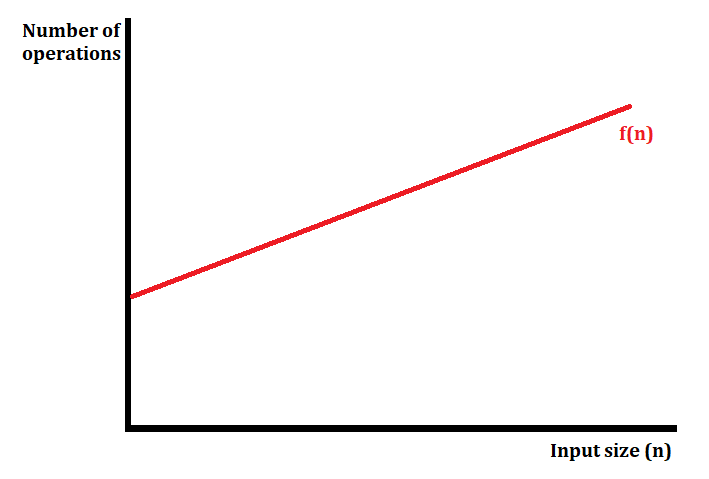
\includegraphics[scale=0.5]{img/graph1.PNG}
\end{center}
Where $f(n)$ describes the number of operations of your algorithm for some $n$. 
\begin{itemize}
    \item We say that $f(n)$ is $O(g(n))$ if, for some constant $a$, we have $a * g(n) \geq f(n)$ as $n \to \infty$. 
    
    \bigskip 

    Consider the following graph: 
    \begin{center}
        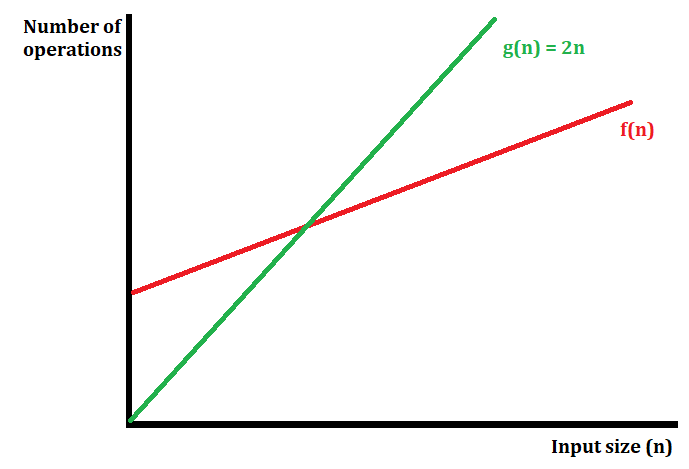
\includegraphics[scale=0.5]{img/graph2.PNG}
    \end{center}
    Here, we see that the intersection of the red and the green line occurs at some point, and that after that point the green line will always be greater than the red line. In other words, at that point, we can say that $f(n)$ will never be bigger than $g(n)$ beyond that point. Therefore, we say that $f(n)$ is $O(2n)$, or simply $O(n)$.
    
    \item Big-$\Omega$ works similarly. We say that $f(n)$ is $\Omega(g(n))$ if, for some constant $b$, $b * g(n) \leq f(n)$ as $n \to \infty$.
    
    \bigskip 

    Consider the following graph: 
    \begin{center}
        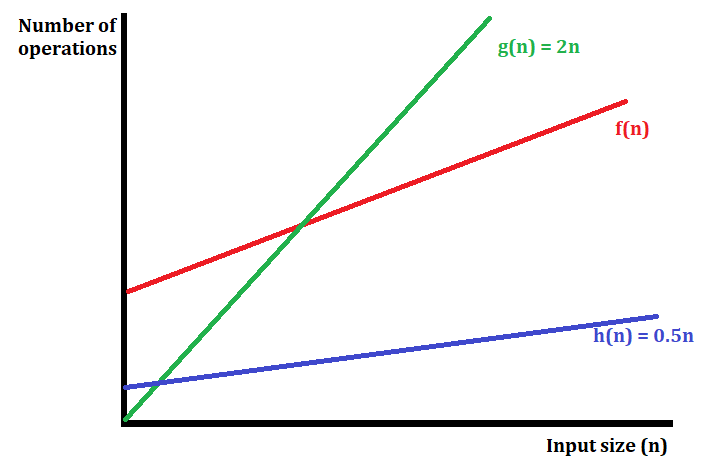
\includegraphics[scale=0.5]{img/graph3.PNG}
    \end{center}
    Here, we see that the blue line $h$ is strictly lower than the red line. In other words, $f(n)$ will never be smaller than $h(n)$. Therefore, we say that $f(n)$ is $\Omega(0.5n)$, or simply $\Omega(n)$. 
    
    \item We say that $f(n)$ is $\Omega(g(n))$ if $f(n)$ is $O(g(n))$ and $f(n)$ is $\Omega(g(n))$. Mathematically: 
    \[b * g(n) \leq f(n) \leq a g(n)\]
    
    In the graphs above, we already found the $b$ and $a$ constants. So:
    \[0.5n \leq f(n) \leq 2n\]
    Therefore, we cn say $f(n)$ is $\Omega(n)$.
\end{itemize}

\textbf{Remarks:} 
\begin{itemize}
    \item Your bigger or smaller functions do not need to be strictly (i.e. always) bigger or smaller than your $f(n)$. They just need to be strictly bigger or smaller beyond some $n$.
    \item We will almost always use Big-$O$. 
\end{itemize}



\end{document}